\documentclass[titlepage]{article}

\usepackage[letterpaper,margin=1in,footskip=0.25in]{geometry}
\usepackage{fancyhdr}
\usepackage{csquotes}
\usepackage{tikz}
\usepackage{mdframed}
\usepackage{amsmath,amssymb}
\usepackage[nottoc,notlof]{tocbibind}
\usepackage{scrextend}
\usepackage{titlesec}
\usepackage{wasysym}
\usepackage{enumitem}
\usepackage[hidelinks]{hyperref}
\usepackage[toc]{glossaries}

\MakeOuterQuote{"}

\newmdenv[
    backgroundcolor=red!10,
    linewidth=0,
    innertopmargin=\topskip,
    innerbottommargin=\topskip
]{probint}
\newmdenv[
    backgroundcolor=yellow!80!red!10,
    linewidth=0,
    innertopmargin=\topskip,
    innerbottommargin=\topskip
]{prob}

\deffootnotemark{\textsuperscript{[\thefootnotemark]}}
\deffootnote[2em]{0em}{1.6em}{\textsuperscript{\thefootnotemark}}

\titleformat*{\subparagraph}{\itshape}

\makeglossaries
\newglossaryentry{markovmatrix}{
    name=markov matrix,
    description={An $n$-square matrix $A$ such that every entry $a_{ij}\in[0,1]$ and the sum of all entries $a_{ij}$ in each column $j$ is 1. Symbolically, $\sum_{i=1}^n a_{ij} = 1$ for all $j=1,2,\dots,n$}
}
\newglossaryentry{markovchain}{
    name=markov chain,
    description={``An algebraic system that experiences transitions from one state to another according to certain probabilistic rules" \cite{bib:markovchains}}
}
\newglossaryentry{diagonalize}{
    name=diagonalize,
    description={To factor an $n$-square matrix $A$ into the form $S\Lambda S^{-1}$, where $S$ is an $n$-square matrix containing the eigenvectors $x_1,x_2,\dots,x_n$ (from left to right) of $A$ and $\Lambda$ is an $n$-square diagonal matrix containing the corresponding eigenvalues $\lambda_1,\lambda_2,\dots,\lambda_n$ (from top-left to bottom-right) of $A$}
}
\newglossaryentry{singular}{
    name=singular,
    description={Not invertible. Other characteristics of singular matrices include not being full column rank and having a nontrivial null space}
}
\newglossaryentry{permutationmatrix}{
    name=permutation matrix,
    description={A matrix with exactly one 1 in every row and column and zeroes everywhere else}
}
\renewcommand{\glsnamefont}{\makefirstuc}

\renewcommand{\labelenumii}{\theenumii.}

\newcounter{lemma}
\newcounter{theorem}

\newenvironment{lemma}[2]{
    \refstepcounter{lemma}\label{#1}
    \paragraph{Lemma \thelemma} #2

    \setlength{\leftskip}{15pt}
    \subparagraph{\hspace{-15pt}Proof}
}{

    \setlength{\leftskip}{0pt}
    \qed
}
\newenvironment{theorem}[2]{
    \refstepcounter{theorem}\label{#1}
    \paragraph{Theorem \thetheorem} #2

    \setlength{\leftskip}{15pt}
    \subparagraph{\hspace{-15pt}Proof}
}{

    \setlength{\leftskip}{0pt}
    \qed
}

\newcommand{\qed}{
    \begin{flushright}
        $\blacksquare$
    \end{flushright}
}
\newcommand{\dd}[2][]{\frac{\text{d}#1}{\text{d}#2}}
\newcommand{\spn}[1]{\text{span}\left( #1 \right)}

\title{On Infinite Markov Chains}
\author{Steven Labalme}
\date{\today}

\begin{document}




\maketitle



\pagenumbering{roman}
\tableofcontents
\listoffigures
\newpage



\pagenumbering{arabic}
\pagestyle{fancy}
\fancyhf{}
\rfoot{Labalme \thepage}
\renewcommand{\headrulewidth}{0pt}
\begin{center}
    \setcounter{secnumdepth}{0}
    \section{Abstract}
    \setcounter{secnumdepth}{3}
\end{center}
This paper was inspired by Problem 9 of the Chapter 6 review problems, which is restated below for convenience.
\vspace{8pt}

\begin{probint}
    \begin{description}
        \item[Problem 9] \hfill \\ Let $
            A =
            \begin{bmatrix}
                0.9 & 0.4\\
                0.1 & 0.6\\
            \end{bmatrix}
        $. Find the limiting value of $
            A^k
            \begin{bmatrix}
                3\\
                2\\
            \end{bmatrix}
        $ as $k\to\infty$.
    \end{description}
\end{probint}

However, to clarify the findings of this paper\footnote{So that $c\neq 1$ in Section \ref{ss2:applying}. If $c$ were to equal 1, the derived-by-inspection null space vector could be confused with the solution vector.}, Problem 9 will hereafter be considered to be the following.

\begin{prob}
    \begin{description}
        \item[Problem 9] \hfill \\ Let $
            A =
            \begin{bmatrix}
                0.9 & 0.4\\
                0.1 & 0.6\\
            \end{bmatrix}
        $. Find the limiting value of $
            A^k
            \begin{bmatrix}
                6\\
                4\\
            \end{bmatrix}
        $ as $k\to\infty$.
    \end{description}
\end{prob}

While Problem 9 presents as a straightforward \Gls{markovchain} problem, and it certainly can be solved as such, this paper explores a quicker, far simpler method. To begin, Problem 9 will be solved by following the standard \Gls{markovchain} procedure. Following that, empirical evidence will be assembled to suggest the presence of a simpler method, and this evidence will be fleshed out into a workable method. After the validity of this new method is shown to extend to Problem 9, the tenets of the method will be rigorously derived.\par
Having been presented, employed, and justified, the new method will be compared and contrasted with the \Gls{markovchain} method. Lastly, a number of new areas of research opened up by the derivation of the new method will be explored.\par
Note that the techniques used in Section \ref{sse:markovchain} are adapted from in-class teachings, summarized in the author's class notes for Chapter 6: \cite{bib:ch6notes}.
\newpage



\section{Solving Problem 9 With a Markov Chain}\label{sse:markovchain}
Restate Problem 9 for convenience:

\begin{prob}
    \begin{description}
        \item[Problem 9] \hfill \\ Let $
            A =
            \begin{bmatrix}
                0.9 & 0.4\\
                0.1 & 0.6\\
            \end{bmatrix}
        $. Find the limiting value of $
            A^k
            \begin{bmatrix}
                6\\
                4\\
            \end{bmatrix}
        $ as $k\to\infty$.
    \end{description}
\end{prob}

The presence of both a \textbf{\Gls{markovmatrix}} ($A$) and of $A$ being raised to a power before mapping an initial condition vector evokes a \textbf{\Gls{markovchain}}. As such, the tools of \Glspl{markovchain} can be employed to evaluate Equation \ref{eqn:problem9}, which symbolically represents Problem 9.

\begin{equation}\label{eqn:problem9}
    \lim_{k\to\infty}
    \begin{bmatrix}
        0.9 & 0.4\\
        0.1 & 0.6\\
    \end{bmatrix}^k
    \begin{bmatrix}
        6\\
        4\\
    \end{bmatrix}
\end{equation}

To efficiently raise $A$ to an arbitrarily high power, \textbf{\gls{diagonalize}} it. The reason for the diagonalization is that due to the nature of the $A=S\Lambda S^{-1}$ factorization, $A^k=S\Lambda^kS^{-1}$. Indeed, diagonalization transforms the complex process of raising $A$ to a power into the extremely simple task of raising a diagonal matrix to a power and then recompiling the factorization.\par
To \gls{diagonalize} $A$, first find the eigenvalues, as follows.
\begin{align*}
    0 &=
    \begin{vmatrix}
        0.9-\lambda & 0.4\\
        0.1 & 0.6-\lambda\\
    \end{vmatrix}\\
    &= (0.9-\lambda)(0.6-\lambda)-(0.4)(0.1)\\
    &= 0.54-1.5\lambda+\lambda^2-0.04\\
    &= \lambda^2-1.5\lambda+0.5\\
    &= 2\lambda^2-3\lambda+1\\
    &= (2\lambda-1)(\lambda-1)
\end{align*}
\begin{align*}
    \lambda_1 &= 0.5&
        \lambda_2 &= 1
\end{align*}
Use the eigenvalues to find the eigenvectors, as follows\footnote{\label{fnt:inspection}Note that the sudden appearance of the eigenvectors in the following algebra is because inspection (basically guess and check) was used to find them. Inspection is a suitable method for simple instances, such as this 2-square example.}.
\begin{align*}
    0 &= (A-\lambda_1I)x_1&
        0 &= (A-\lambda_2I)x_2\\
    \begin{bmatrix}
        0\\
        0\\
    \end{bmatrix}    
    &= \left( 
        \begin{bmatrix}
            0.9 & 0.4\\
            0.1 & 0.6\\
        \end{bmatrix}
        -0.5
        \begin{bmatrix}
            1 & 0\\
            0 & 1\\
        \end{bmatrix}
    \right)
    \begin{bmatrix}
        x_{1_1}\\
        x_{1_2}\\
    \end{bmatrix}&
        \begin{bmatrix}
            0\\
            0\\
        \end{bmatrix}
        &= \left( 
            \begin{bmatrix}
                0.9 & 0.4\\
                0.1 & 0.6\\
            \end{bmatrix}
            -1
            \begin{bmatrix}
                1 & 0\\
                0 & 1\\
            \end{bmatrix}
        \right)
        \begin{bmatrix}
            x_{1_1}\\
            x_{1_2}\\
        \end{bmatrix}\\
    &=
    \begin{bmatrix}
        0.4 & 0.4\\
        0.1 & 0.1\\
    \end{bmatrix}
    \begin{bmatrix}
        x_{1_1}\\
        x_{1_2}\\
    \end{bmatrix}&
        &=
        \begin{bmatrix}
            -0.1 & 0.4\\
            0.1 & -0.4\\
        \end{bmatrix}
        \begin{bmatrix}
            x_{1_1}\\
            x_{1_2}\\
        \end{bmatrix}\\
    &=
    \begin{bmatrix}
        0.4 & 0.4\\
        0.1 & 0.1\\
    \end{bmatrix}
    \begin{bmatrix}
        -1\\
        1\\
    \end{bmatrix}&
        &=
        \begin{bmatrix}
            -0.1 & 0.4\\
            0.1 & -0.4\\
        \end{bmatrix}
        \begin{bmatrix}
            4\\
            1\\
        \end{bmatrix}
\end{align*}
\begin{align*}
    x_1 &=
    \begin{bmatrix}
        -1\\
        1\\
    \end{bmatrix}&
        x_2 &=
        \begin{bmatrix}
            4\\
            1\\
        \end{bmatrix}
\end{align*}
From the above information ($\lambda_1$, $\lambda_2$, $x_1$, and $x_2$), $A$ can be diagonalized as follows\footnote{Note that the $-\frac{1}{5}$ pertains to every entry of $S^{-1}$. It is factored out so that every entry of $S^{-1}$ is not a decimal.}.

\begin{equation}\label{eqn:diagonalization}
    A = -\frac{1}{5}
    \begin{bmatrix}
        -1 & 4\\
        1 & 1\\
    \end{bmatrix}
    \begin{bmatrix}
        0.5 & 0\\
        0 & 1\\
    \end{bmatrix}
    \begin{bmatrix}
        1 & -4\\
        -1 & -1\\
    \end{bmatrix}
\end{equation}

At this point, it is possible to return to the original task of evaluating Equation \ref{eqn:problem9}. Begin by substituting Equation \ref{eqn:diagonalization} into Equation \ref{eqn:problem9}, as follows.
\begin{equation*}
    \lim_{k\to\infty}
    \left( 
        -\frac{1}{5}
        \begin{bmatrix}
            -1 & 4\\
            1 & 1\\
        \end{bmatrix}
        \begin{bmatrix}
            0.5 & 0\\
            0 & 1\\
        \end{bmatrix}
        \begin{bmatrix}
            1 & -4\\
            -1 & -1\\
        \end{bmatrix}
    \right)^k
    \begin{bmatrix}
        6\\
        4\\
    \end{bmatrix}
\end{equation*}
As was discussed earlier, move the exponent into the factorization so that it only raises $\Lambda$ to the power $k$.
\begin{equation*}
    \lim_{k\to\infty} -\frac{1}{5}
    \begin{bmatrix}
        -1 & 4\\
        1 & 1\\
    \end{bmatrix}
    \begin{bmatrix}
        0.5 & 0\\
        0 & 1\\
    \end{bmatrix}^k
    \begin{bmatrix}
        1 & -4\\
        -1 & -1\\
    \end{bmatrix}
    \begin{bmatrix}
        6\\
        4\\
    \end{bmatrix}
\end{equation*}
Apply the fact that raising a diagonal matrix to a power is the same as raising each of its entries to that power.
\begin{equation*}
    \lim_{k\to\infty} -\frac{1}{5}
    \begin{bmatrix}
        -1 & 4\\
        1 & 1\\
    \end{bmatrix}
    \begin{bmatrix}
        0.5^k & 0\\
        0 & 1^k\\
    \end{bmatrix}
    \begin{bmatrix}
        1 & -4\\
        -1 & -1\\
    \end{bmatrix}
    \begin{bmatrix}
        6\\
        4\\
    \end{bmatrix}
\end{equation*}
It is now possible to evaluate the limit. While it is not be obvious what limit the entirety of the above expression approaches, all that is necessary is to evaluate the limits of $0.5^k$ and $1^k$ as $k\to\infty$, respectively, and then recompile the factorization. This can be done as follows.
\begin{align*}
    \lim_{k\to\infty} -\frac{1}{5}
    \begin{bmatrix}
        -1 & 4\\
        1 & 1\\
    \end{bmatrix}
    \begin{bmatrix}
        0.5^k & 0\\
        0 & 1^k\\
    \end{bmatrix}
    \begin{bmatrix}
        1 & -4\\
        -1 & -1\\
    \end{bmatrix}
    \begin{bmatrix}
        6\\
        4\\
    \end{bmatrix}
    &= -\frac{1}{5}
    \begin{bmatrix}
        -1 & 4\\
        1 & 1\\
    \end{bmatrix}
    \begin{bmatrix}
        0 & 0\\
        0 & 1\\
    \end{bmatrix}
    \begin{bmatrix}
        1 & -4\\
        -1 & -1\\
    \end{bmatrix}
    \begin{bmatrix}
        6\\
        4\\
    \end{bmatrix}\\
    &= -\frac{1}{5}
    \begin{bmatrix}
        -1 & 4\\
        1 & 1\\
    \end{bmatrix}
    \begin{bmatrix}
        0 & 0\\
        0 & 1\\
    \end{bmatrix}
    \begin{bmatrix}
        -10\\
        -10\\
    \end{bmatrix}\\
    &= -\frac{1}{5}
    \begin{bmatrix}
        -1 & 4\\
        1 & 1\\
    \end{bmatrix}
    \begin{bmatrix}
        0\\
        -10\\
    \end{bmatrix}\\
    &= -\frac{1}{5}
    \begin{bmatrix}
        -40\\
        -10\\
    \end{bmatrix}\\
    &=
    \begin{bmatrix}
        8\\
        2\\
    \end{bmatrix}
\end{align*}
The vector $
    \begin{bmatrix}
        8\\
        2\\
    \end{bmatrix}
$ is the final simplification of Equation \ref{eqn:problem9} and, therefore, the answer to Problem 9.
\newpage



\section{Solving Problem 9 More Concisely}
\subsection{A New Method}
\subsubsection{Assembling the New Method}\label{ss2:assemble}
The limit given by Equation \ref{eqn:problem9} converges on an element of $\mathbb{R}^2$ as $k\to\infty$. But there is another, simpler way to think about this process. Because the limit converges, as $k$ increases, the change that each repeated application of $A$ causes to the product diminishes, i.e., the difference vector $Ax_0-x_0$ is greater in magnitude than the difference vector $A^2x_0-Ax_0$, and so on and so forth.\par
The consistently diminishing nature of the difference vector implies that at infinity, this difference vector is 0: symbolically, $AA^\infty x_0-A^\infty x_0=0$. If $x=A^\infty x_0$ is the solution vector (the evaluation of Equation \ref{eqn:problem9}), then substitution gives $Ax-x=0$, or
\begin{equation}\label{eqn:Axx}
    Ax = x
\end{equation}
This result actually makes quite a bit of sense --- if $x$ truly is the limit of repeated multiplications by $A$, it stands to reason that $A$ could no longer do anything to change it. Indeed, $A$ would be an identity map on $x$, and the above equation reflects that fact, as it can be restated $Ax=Ix$.\par
Equation \ref{eqn:Axx} provides a computationally far simpler method than Markov chains to find $x$. However, the solution to $Ax=x$ is the one-dimensional subspace $\spn{x}$, only one vector of which will be the solution to Problem 9. Thus, to pin down a single vector, it will be necessary to find a second equation describing this situation.\par
A good first place to look is at the initial conditions $x_0$, which have not yet been used. Since the solution most certainly depends on them, perhaps it is possible to use them to find the desired vector of $\spn{x}$, killing two birds with one stone. Indeed, finding a single solution depends on the initial conditions, but in a manner best visualized by applying the \Gls{markovchain} to a more tangible model, as follows.

\begin{figure}[h!]
    \centering
    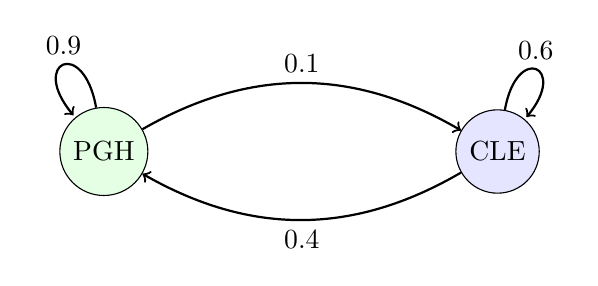
\begin{tikzpicture}[
        every path/.style={thick,->}
    ]
        \node [circle,draw,thin,fill=green!10] (PGH) {PGH}
            edge [out=100,in=130,loop] node[above]{0.9} ()
        ;
        \node [circle,draw,thin,fill=blue!10] (CLE) at (5,0) {CLE}
            edge [out=80,in=50,loop] node[above]{0.6} ()
        ;
        
        \draw (PGH) to[bend left=30] node[above]{0.1} (CLE);
        \draw (CLE) to[bend left=30] node[below]{0.4} (PGH);
    \end{tikzpicture}
    \caption{Modeling population changes with a Markov chain.}
    \label{fig:population}
\end{figure}

Consider matrix $A$ from Problem 9, but with the initial conditions adjusted to be 600,000 and 400,000 respectively. Figure \ref{fig:population} visualizes Problem 9 in the following ways.
\begin{enumerate}[itemsep=0pt]
    \item Imagine that 600,000 is the population of Pittsburgh (PGH) in year 0.
    \item Imagine that 400,000 is the population of Cleveland (CLE) in year 0.
    \begin{enumerate}
        \item Together, the populations are represented by the vector $
            x_0 =
            \begin{bmatrix}
                \text{PGH}\\
                \text{CLE}\\
            \end{bmatrix}
            =
            \begin{bmatrix}
                600,000\\
                400,000\\
            \end{bmatrix}
        $.
    \end{enumerate}
    \item Every year, 90\% (0.9) of Pittsburgh's population remains in Pittsburgh, and 10\% (0.1) moves to Cleveland.
    \item Every year, 60\% (0.6) of Cleveland's population remains in Cleveland, and 40\% (0.4) make the right choice (\smiley{}).
    \begin{enumerate}
        \item Together, the movements are represented by the linear map $
            A =
            \begin{bmatrix}
                0.9 & 0.4\\
                0.1 & 0.6\\
            \end{bmatrix}
        $.
    \end{enumerate}
    \item In year $k$, the populations of each city are given by $A^kx_0$.
    \begin{enumerate}
        \item For example, in year 1, the populations are $
            \begin{bmatrix}
                \text{PGH}\\
                \text{CLE}\\
            \end{bmatrix}
            = A^1x_0 =
            \begin{bmatrix}
                0.9 & 0.4\\
                0.1 & 0.6\\
            \end{bmatrix}^1
            \begin{bmatrix}
                600,000\\
                400,000\\
            \end{bmatrix}
            =
            \begin{bmatrix}
                700,000\\
                300,000\\
            \end{bmatrix}
        $.
    \end{enumerate}
    \item In the long run, the populations of each city are given by the limit of $A^kx_0$ as $k\to\infty$.
    \begin{enumerate}
        \item Eventually, the populations converge on $
            \begin{bmatrix}
                \text{PGH}\\
                \text{CLE}\\
            \end{bmatrix}
            = A^\infty x_0 =
            \begin{bmatrix}
                0.9 & 0.4\\
                0.1 & 0.6\\
            \end{bmatrix}^\infty
            \begin{bmatrix}
                600,000\\
                400,000\\
            \end{bmatrix}
            =
            \begin{bmatrix}
                800,000\\
                200,000\\
            \end{bmatrix}
        $\footnote{Note that the final vector can be found by scaling the solution vector from Section \ref{sse:markovchain} by the same factor (100,000) that scaled $x_0$. This is further evidence that the solution depends on the initial conditions.}.
    \end{enumerate}
\end{enumerate}
In this model, it should be clear that no person is ever introduced or removed from the system --- they only move from one city to the other, or stay in place. This is reflected by the fact that the net number of people in every "year" given above is always one million --- $600,000+400,000=1,000,000$, $700,000+300,000=1,000,000$, and $800,000+200,000=1,000,000$.\par
Herein lies the key: Multiplying the initial conditions by a \Gls{markovmatrix} $A$ appears to preserve the sum of the values in $x_0$. Therefore, it is possible to formalize this second rule as follows, where each sum iterates through the $n$ entries in its respective vector.
\begin{equation}\label{eqn:sum}
    \sum_{i=1}^n x_{0_i} = \sum_{i=1}^n x_i
\end{equation}
With the results of Equations \ref{eqn:Axx} and \ref{eqn:sum}, solving Problem 9 is a trivial matter.

\subsubsection{Applying the New Method}\label{ss2:applying}
Restate Problem 9 for convenience:

\begin{prob}
    \begin{description}
        \item[Problem 9] \hfill \\ Let $
            A =
            \begin{bmatrix}
                0.9 & 0.4\\
                0.1 & 0.6\\
            \end{bmatrix}
        $. Find the limiting value of $
            A^k
            \begin{bmatrix}
                6\\
                4\\
            \end{bmatrix}
        $ as $k\to\infty$.
    \end{description}
\end{prob}

In parallel with Section \ref{ss2:assemble}, $A$ is a 2-square \Gls{markovmatrix} and $x_0$ will be the variable name for the initial conditions of the \Gls{markovchain} in Problem 9. Also, once again let $x$ be the sought-after solution vector.\par
Use Equation \ref{eqn:Axx} to solve for the subspace in which $x$ lies (see Footnote \ref{fnt:inspection}).
\begin{align*}
    x &= Ax\\
    0 &= Ax-x\\
    &= Ax-Ix\\
    &= (A-I)x\\
    \begin{bmatrix}
        0\\
        0\\
    \end{bmatrix}
    &= \left( 
        \begin{bmatrix}
            0.9 & 0.4\\
            0.1 & 0.6\\
        \end{bmatrix}
        -
        \begin{bmatrix}
            1 & 0\\
            0 & 1\\
        \end{bmatrix}
    \right)
    \begin{bmatrix}
        x_1\\
        x_2\\
    \end{bmatrix}\\
    &=
    \begin{bmatrix}
        -0.1 & 0.4\\
        0.1 & -0.4\\
    \end{bmatrix}
    \begin{bmatrix}
        x_1\\
        x_2\\
    \end{bmatrix}\\
    &=
    \begin{bmatrix}
        -0.1 & 0.4\\
        0.1 & -0.4\\
    \end{bmatrix}
    \begin{bmatrix}
        4c\\
        1c\\
    \end{bmatrix}
    ,\qquad c\in\mathbb{R}
\end{align*}

\begin{equation*}
    x = \spn{
        \begin{bmatrix}
            4\\
            1\\
        \end{bmatrix}
    }
\end{equation*}
Use Equation \ref{eqn:sum} to solve for a single $x$.
\begin{align*}
    \sum_{i=1}^n x_{0_i} &= \sum_{i=1}^n x_i\\
    6+4 &= 4c+1c\\
    c &= 2
\end{align*}
\begin{align*}
    x &=
    \begin{bmatrix}
        4(2)\\
        1(2)\\
    \end{bmatrix}\\
    &=
    \begin{bmatrix}
        8\\
        2\\
    \end{bmatrix}
\end{align*}
The vector $
    \begin{bmatrix}
        8\\
        2\\
    \end{bmatrix}
$ is the specific element of $
    \spn{
        \begin{bmatrix}
            4\\
            1\\
        \end{bmatrix}
    }
$ that is the solution to Problem 9.


\subsection{Rigorously Deriving the New Method}\label{sss:rigorous}
Let $A$ be an $n$-square \Gls{markovmatrix}, and let $x_0$ be a vector of initial conditions for the \Gls{markovchain}.

\begin{lemma}{lma:A-I}{
    $A-I$ is a \textbf{\gls{singular}} matrix.
}
    By the definition of a \gls{markovmatrix}, the entries in each column of $A$ sum to 1. However, when the difference $A-I$ is taken, one entry of every column of $A$ decreases in value by 1. Thus, the entries in each column of $A-I$ sum to 0.\par
    If the sum of the entries in each column of $A-I$ is 0, every column $j$ (and every vector $v\in C(A)$) can be expressed in the following form.
    \begin{equation*}
        v =
        \begin{bmatrix}
            a_{1j}\\
            a_{2j}\\
            \vdots\\
            a_{(n-1)j}\\
            -a_{1j}-a_{2j}-\cdots-a_{(n-1)j}\\
        \end{bmatrix}
    \end{equation*}
    Notably, no vector \emph{not} in this form can be an element of $C(A-I)$, and, similarly, any vector not in this form would be an element of $N(A-I)$. Thus, proving that $A-I$ is \gls{singular} becomes a task of finding a vector $u\in\mathbb{R}^n$ that is not in the above form. The following is an example of such a vector.
    \begin{equation*}
        u =
        \begin{bmatrix}
            1\\
            1\\
            \vdots\\
            1\\
        \end{bmatrix}
    \end{equation*}
    It is obvious that the above vector is not in the form necessary for it to be an element of $C(A-I)$.\par
    However, as further proof that $u\notin C(A-I)$ and $u\in N(A-I)$, the fundamental theorem of linear algebra asserts that all elements of $C(A-I)$ are orthogonal to all elements of $N(A-I)$, or, alternatively, that the dot product of any element of the column space with any element of the null space is 0. Since $v$ encapsulates every possible element of $C(A)$, the following definitively proves that $u\notin C(A)$.
    \begin{align*}
        0 &= v\cdot u\\
        &=
        \begin{bmatrix}
            a_{1j}\\
            a_{2j}\\
            \vdots\\
            a_{(n-1)j}\\
            -a_{1j}-a_{2j}-\cdots-a_{(n-1)j}\\
        \end{bmatrix}
        \cdot
        \begin{bmatrix}
            1\\
            1\\
            \vdots\\
            1\\
        \end{bmatrix}\\
        &= (1)(a_{1j})+(1)(a_{2j})+\cdots+(1)(a_{(n-1)j})+(1)(-a_{1j}-a_{2j}-\cdots-a_{(n-1)j})\\
        &= 0
    \end{align*}
    Since there always exist elements of $\mathbb{R}^n$ (at least $\spn{u}$) in $N(A-I)$, $A-I$ is \gls{singular}.
\end{lemma}

\begin{lemma}{lma:Axx}{
    For any $A$, there exists a vector $x$ satisfying $Ax=x$.
}
    By Lemma \ref{lma:A-I}, the matrix $A-I$ has a null space. In other words, the following equation has at least one family of solutions.
    \begin{equation*}
        (A-I)x = 0
    \end{equation*}
    The above equation can be algebraically rearranged as follows, proving the lemma.
    \begin{align*}
        (A-I)x &= 0\\
        Ax-Ix &= 0\\
        Ax &= Ix\\
        Ax &= x
    \end{align*}
\end{lemma}

Lemmas \ref{lma:A-I} and \ref{lma:Axx} hold true for any \Gls{markovmatrix} $A$. However, before tackling convergence, it is necessary to point out that not all \Glspl{markovchain} converge. For example, if $A$ is the following \textbf{\gls{permutationmatrix}}, the \Gls{markovchain} diverges periodically for some $x_0\in\mathbb{R}^n$.

\begin{equation*}
    \begin{bmatrix}
        0 & 1 & 0\\
        1 & 0 & 0\\
        0 & 0 & 1\\
    \end{bmatrix}
\end{equation*}

\begin{theorem}{trm:xislimit}{
    The solution to $\lim_{k\to\infty}A^kx_0$ lies in $\spn{x}$, where $x$ satisfies $Ax=x$, for any $x_0\in\mathbb{R}^n$ if and only if the limit converges.
}
    If $\lim_{k\to\infty}A^kx_0$ converges, the difference vector $A^{k+1}x_0-A^kx_0$ between an instance $A^kx_0$ and the next instance $A^{k+1}x_0$ converges to 0. The convergence of the distance vector implies the validity of the following algebra.
    \begin{align*}
        0 &= \lim_{k\to\infty} \left( A^{k+1}x_0-A^kx_0 \right)\\
        &= \lim_{k\to\infty} \left( AA^kx_0-IA^kx_0 \right)\\
        &= \lim_{k\to\infty} (A-I)A^kx_0\\
        &= (A-I)\lim_{k\to\infty} A^kx_0
    \end{align*}\par
    By the above algebra, $\lim_{k\to\infty} A^kx_0$ is an element of $N(A-I)$. If $\lim_{k\to\infty} A^kx_0\in N(A-I)$, Lemma \ref{lma:Axx} guarantees that it lies in $\spn{x}$, where $x$ satisfies $Ax=x$. 
\end{theorem}

Theorem \ref{trm:xislimit} concludes the proof of Equation \ref{eqn:Axx}. All that is left at this point is to prove Equation \ref{eqn:sum}.

\begin{lemma}{lma:sum}{
    The sum of the entries in $x_0$ equals the sum of the entries in $Ax_0$. Symbolically, the following equation is true for any $A$ and $x_0$: $\sum_{i=1}^nx_{0_i}=\sum_{i=1}^n\left( Ax_0 \right)_i$.
}
    Let $A$ and $x_0$ be visualized as follows.
    \begin{align*}
        A &=
        \begin{bmatrix}
            a_{11} & a_{12} & \cdots & a_{1n}\\
            a_{21} & a_{22} & \cdots & a_{2n}\\
            \vdots & \vdots & \ddots & \vdots\\
            a_{n1} & a_{n2} & \cdots & a_{nn}\\
        \end{bmatrix}&
            x_0 &=
            \begin{bmatrix}
                x_{0_1}\\
                x_{0_2}\\
                \vdots\\
                x_{0_n}
            \end{bmatrix}
    \end{align*}
    Then $Ax_0$ is given by the following.
    \begin{align*}
        Ax_0 &=
        \begin{bmatrix}
            a_{11} & a_{12} & \cdots & a_{1n}\\
            a_{21} & a_{22} & \cdots & a_{2n}\\
            \vdots & \vdots & \ddots & \vdots\\
            a_{n1} & a_{n2} & \cdots & a_{nn}\\
        \end{bmatrix}
        \begin{bmatrix}
            x_{0_1}\\
            x_{0_2}\\
            \vdots\\
            x_{0_n}\\
        \end{bmatrix}\\
        &=
        \begin{bmatrix}
            a_{11}x_{0_1}+a_{12}x_{0_2}+\cdots+a_{1n}x_{0_n}\\
            a_{21}x_{0_1}+a_{22}x_{0_2}+\cdots+a_{2n}x_{0_n}\\
            \vdots\\
            a_{n1}x_{0_1}+a_{n2}x_{0_2}+\cdots+a_{nn}x_{0_n}\\
        \end{bmatrix}
    \end{align*}
    With both $x_0$ and $Ax_0$ defined, algebraically transform one of the expressions in the hypothesis into the other, as follows.
    \begin{align*}
        \sum_{i=1}^n\left( Ax_0 \right)_i &= (a_{11}x_{0_1}+\cdots+a_{1n}x_{0_n})+(a_{21}x_{0_1}+\cdots+a_{2n}x_{0_n})+\cdots+(a_{n1}x_{0_1}+\cdots+a_{nn}x_{0_n})\\
        &= (a_{11}+\cdots+a_{n1})x_{0_1}+(a_{12}+\cdots+a_{n2})x_{0_2}+\cdots+(a_{1b}+\cdots+a_{nb})x_{0_n}\\
        &= 1x_{0_1}+1x_{0_2}+\cdots+1a_{0_n}\\
        &= \sum_{i=1}^nx_{0_i}
    \end{align*}
\end{lemma}

\begin{theorem}{trm:suminduction}{
    The sum of the entries in $x_0$ equals the sum of the entries in $A^kx_0$ for any $k\in\mathbb{N}$.
}
    The following will be an induction proof.\\
    Basis step: $\sum_{i=1}^n (Ax_0)_i \stackrel{\checkmark}{=} \sum_{i=1}^n x_{0_i}$ (guaranteed by Lemma \ref{lma:sum}).\\
    Induction hypothesis: $\sum_{i=1}^n (A^kx_0)_i = \sum_{i=1}^n x_{0_i}$.\\
    Induction step:
    \begin{align*}
        \sum_{i=1}^n (A^{k+1}x_0)_i &\stackrel{?}{=} \sum_{i=1}^n (Ax_0)_i\\
        \sum_{i=1}^n (AA^kx_0)_i &\stackrel{?}{=} \sum_{i=1}^n (Ax_0)_i\\
        \sum_{i=1}^n (Ax_0)_i &\stackrel{\checkmark}{=} \sum_{i=1}^n (Ax_0)_i
    \end{align*}
\end{theorem}

Although Theorem \ref{trm:suminduction} does not directly treat the infinite case, by stating that the sum of the entries never changes under repeated multiplications by $A$, it implies that the sum of the entries never changes as $k\to\infty$, proving Equation \ref{eqn:sum}.\par
Together, Theorems \ref{trm:xislimit} and \ref{trm:suminduction} guarantee that the method of solving Problem 9 used in Section \ref{ss2:applying} stands on solid logical footing.
\newpage



\section{Comparing and Contrasting the Two Methods}
\Glspl{markovchain} are useful not only for their prediction of long-run behavior, but for their prediction of short-term behavior, too. For example, in the population model discussed in association with Figure \ref{fig:population}, the model's 1, 2, or 5-year predictions are likely far more useful than its long-run behavior; after all, those rates of population movement are unlikely to remain static for infinitely many years.\par
However, when determining the long-run behavior of a convergent \Gls{markovchain}, the new method is more than useful. It eliminates the need for the time-consuming process of diagonalization, removes the need for limits entirely, and avoids the lengthy process of recompiling the factorization. Its only flaw, per se, is in its logical footing. The behavior of systems at infinity is difficult to reconcile, and while the results utilized by the new method are all rigorously derived in Section \ref{sss:rigorous}, the logic lacks the benefits of centuries of peer-review and fine tuning that \Glspl{markovchain} have been subjected to.\par
Despite its novelty, the new method is a gateway to discovering and proving fascinating results on the nature of infinite \Glspl{markovchain}, some of which are discussed in the next section.
\newpage



\section{Diving Deeper}
\textcolor{red}{\textit{Coming soon!}}
\newpage



\printglossaries
\newpage



\bibliography{MarkovMeditations}
\bibliographystyle{apalike}




\end{document}